% !TEX root = ../main.tex
% (this is to make TexShop know where your parent file is)
% Further Comments section - for instance as below :


% All of the tracks are mastered for Spotify standard and checked using the Loudness Penalty Analyzer\autocite{loudness:penalty}
% here's how to add an image ... (put images in the images folder. you don't need to add an extension, just the file name)

% \begin{figure}[ht]

%     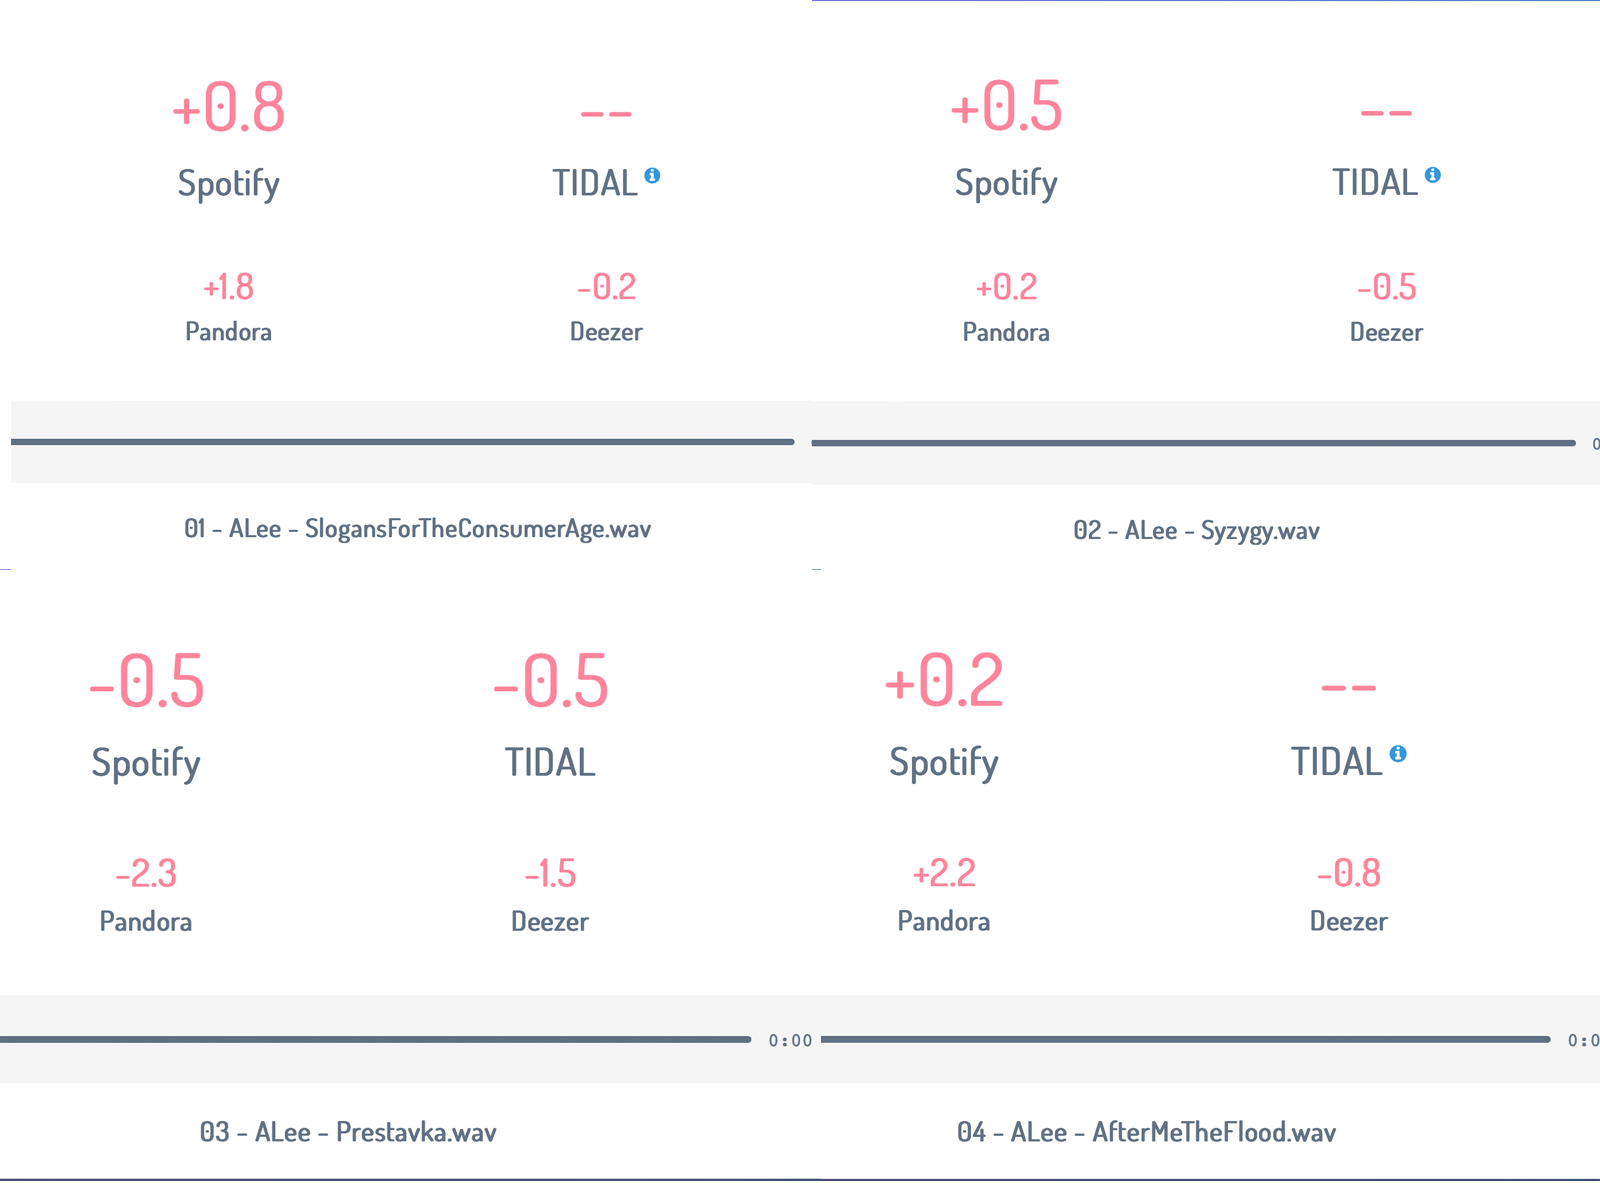
\includegraphics[scale=0.8, width=\textwidth]{images/spotify}
%     \caption{Loudness Penalty Analyzer Results}
%     \label{fig:loudness}
% \end{figure}

This is my first time recording sung vocals, both as an engineer and as a performer, and my first time producing vocals. As I'm also not a very experienced singer, the result isn't quite up to a professional standard, but as a learning experience, I think it has been very valuable.

The same can be said for the few vocal production tips I picked up. Of course, still a long way to go, but valuable learning nonetheless.

And yes, some of the instrumental recordings are a little sloppy, the mix is sorely lacking, and there could have been more and stronger transitions, but this is a formative and I'm running out of time, so I'll take it.

\subsection*{But does it actually work?}

I'm not entirely convinced that this is the right approach for this cutscene. I think it definitely \textit{can} work, but there's too much fighting with the SFX after the sword shatter [01:26], especially. What often happens in these scenes (including in the \textit{Arcane} episode) is that that the music almost completely takes over the soundstage and most SFX are muted or turned down (and kept out of the lower frequencies). This gives the music room to breathe and not have to worry about clashing with the sound effects. However, I didn't know if that would be a viable approach in this assignment \footnote{Technically, the brief doesn't state that you \textit{can't} change it, but I feel like the point is to work with what you've got and not modify what would be other people's work.}

I think there's a couple solutions that could work very well here. The one that would allow the music to shine the most would be to mute the SFX after the shatter and until the mask making [01:53--02:07], and at that point, leave out the heartbeats.

Another option would be to keep the song up until that point --- potentially also over the quiet part before the breakage --- but go into more typical film scoring once the sword breaks (or leave the score out entirely at that point). It could be brought back again after the knight falls to the ground [02:08]. Moving the restatement of the B section [01:53--02:07] to this point would work well.

Overall, I don't think I've successfully stayed out of the way of the SFX here. But I had an idea and I wanted to see it through to its conclusion.
